\documentclass{beamer}

\usetheme{Warsaw}
%% \usetheme{EastLansing}
%% \usecolortheme{beetle}

\title[Functional Programming]{An Introduction to Functional Programming}
\author{Andreas Pauley -- @apauley}
\institute{Pattern Matched Technologies\\Lambda Luminaries}
\date{September 2, 2013}

\usepackage[utf8]{inputenc}
\usepackage{graphicx}

\usepackage{hyperref}

\begin{document}

\begin{frame}
\titlepage
\end{frame}

\begin{frame}{Pattern Matched Technologies}
Developing financial applications in Erlang.
\end{frame}

\begin{frame}{Lambda Luminaries}
\framesubtitle{Local functional programming user group}
We meet once a month, on the second Monday of the month.

\url{http://www.meetup.com/lambda-luminaries/}
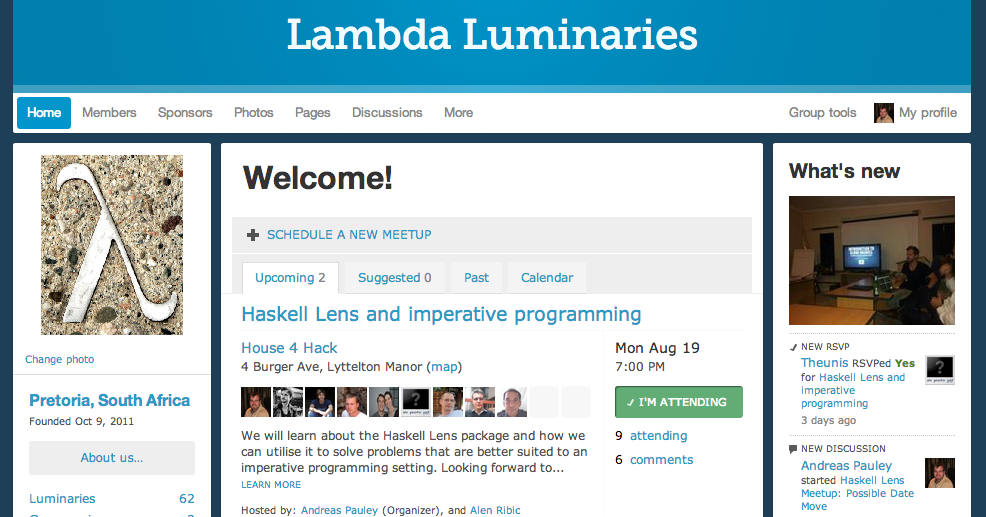
\includegraphics[scale=0.3]{img/LambdaLuminariesScreenShot2013-08-09.png}

\end{frame}

\begin{frame}{A word from the Wise}

\begin{exampleblock}{}
  {\large ``
No matter what language you work in, programming
in a functional style provides benefits.
You should do it whenever it is convenient, and you
should think hard about the decision when it isn’t convenient.
  ''}
  \vskip5mm
  \hspace*\fill{\small--- John Carmack, ID Software}
\end{exampleblock}


\url{http://www.altdevblogaday.com/2012/04/26/functional-programming-in-c/}

\end{frame}


\end{document}
